\documentclass[letter,12pt]{article}
\usepackage[utf8]{inputenc}
\usepackage{fullpage}
\usepackage{graphicx}
\usepackage{caption}
\usepackage{subcaption}
\usepackage{datetime}
\usepackage{indentfirst}
\usepackage{wasysym}
\usepackage{placeins}

\newdateformat{mydate}{\THEDAY\space \shortmonthname[\THEMONTH] \THEYEAR}

\usepackage[backend=biber,maxbibnames=99,defernumbers=true]{biblatex}
	\addbibresource[datatype=bibtex]{./Bibliography.bib}

\begin{document}

%\maketitle

\begin{flushleft}
	\begin{tabular}{l l}
		To: & Prof. Todd Kaiser \\
		From: & Sam Harkness \\
		Regarding: & EELE408 Final Report \\
		Date: & \mydate\today
	\end{tabular}
\end{flushleft}

\begin{abstract}
	This lab report details the theory and process behind fabricating photovoltaic cells on a silicon wafer.  
\end{abstract}

\section{Background}
	\subsection{Fabrication Sequence}\label{sec:Fab_Sequence}
	
		Solar cells are fabricated using a combination of thin film and bulk silicon processing techniques.  The sequence is a simple set of repeating steps including oxidation, etching, diffusion, cleaning, and patterning.  
	
		\subsubsection{Diffusion}
			\FloatBarrier
			Diffusion is a method by which doped regions of silicon are created.  A region is infused with dopants using heat and a source of dopant atoms.  In the case of wanting to create a P type silicon, our process uses Boron. In the case of N type silicon, Phosphorous is used. There are many options for dopants, but Boron and Phosphorous are some of the easier and cheaper to obtain.
			
		  	The sheet resistance can be measured using a four-point probe, as depicted in Figure~\ref{fig:Four_Point_Probe}.
			
			\begin{figure}[h!]
				\centering
				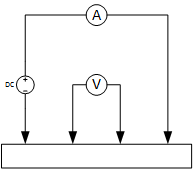
\includegraphics[scale=1]{./Images/Four_Point_Probe.png}
				\caption{Schematic of a Four-Point Probe}
				\label{fig:Four_Point_Probe}
			\end{figure}
		
		\subsubsection{Oxidation}\label{sec:Oxidation}
			\FloatBarrier
			Oxidation is the process by which an insulator is grown on a substrate; in our case Silicon Dioxide SiO$_2$ on Silicon Si. Oxidation can be performed using either a \textit{wet} or \textit{dry} process, utilizing Oxygen O$_2$ or Water H$_2$O respectively. Wet oxidation produces a worse insulator, but grows much faster.  Dry oxidation produces a better insulator, but grows much slower. 
			
			Oxide thickness can be measured using a nanospec, which utilized the reflection and refraction properties of light.
			
		\subsubsection{Photolithography}
			Photolithography is the process by which a mask is transmitted onto the surface of a wafer.  Photolithography is used in every step of wafer fabrication, such as oxidation, diffusion, and metal deposition. 
			
			The photoresist used in our photolithography process is Shipley 1813, a positive resist.  A positive resist is washed away in developer when exposed, whereas a negative resist is washed away in developer when not exposed. A mask is designed to be used with a certain type of resist. For this process, we use 1 $\mu$m of Shipley 1813, requiring an exposure time of 4.5 sec. To distribute an even coating of 1 $\mu$m resist, the wafer is spun at 5250 RMP for 30 sec. \cite{Shipley_1800}
		
		\subsubsection{Etching and Cleaning}
			Our process uses wet etching remove unwanted material, such as oxide or aluminum. SiO$_2$ is etched with Buffered Oxide Etch (BOE), a combination of hydrofluoric acid (HF) and buffering chemicals to stabilize the reaction. BOE is highly selective to silicon dioxide so the photoresist is not etched.  Aluminum (Al) is etched by Phosphoric Acid Etch (PAE) at approximately 350 \AA/min. \cite{407_Lab_Manual} Silicon is etched by Tetramethylammonium Hydroxide (TMAH) at approximately 21.5 $\mu$m/hr. \cite{408_Lab_Manual}
			
			After etching SiO$_2$, Al, or Si, the remaining photoresist is removed using a 3 solvent clean: Acetone, Isopropyl Alcohol, and Methanol. The acetone removes the photoresist, while isopropyl and methanol remove acetone residue. Finally, the wafers are rinsed with deionized water and dried with nitrogen. This removes errant dust particles from the surface of the wafer. \cite{407_Lab_Manual}
			
			Before a deposition, an RCA clean is performed. The RCA clean consists of 3 chemical solutions.  The first is a mixture of sulfuric acid and hydrogen peroxide, known as a Pirahna etch, that removes organic materials.  The second is a weak BOE to strip native oxide.  The final mixture, ionic clean, removes heavy metal ions with hydrochloric acid, water, and hydrogen peroxide. \cite{407_Lab_Manual}
			
			Etching can be either isotropic or anisotropic.  An isotropic etch etches in all directions equally, creating a 'spherical' pit in the surface of a material through an opening.  An anisotropic etch, however, may etch at differing rates depending on a number of factors.  In the case of a dry etch, such as plasma, ions are being directed at a certain angle, so the etching happens in that direction.  In the case of a wet etch, the crystal planes of a material can influence the direction of the etch.
		
		\subsubsection{Metal Evaporation}
			The method of depositing a conductor for this process is Physical Vapor Deposition (PVD). In our case, Aluminum (Al) is the conductor of choice. In PVD, the conductive material is evaporated using heat and condenses on the surface of the wafer.  Using simple geometry, the thickness of the Al can be determined for any point on the wafer.			
		
	\subsection{Fabrication Sequence}
		\FloatBarrier
		The general sequence in CMOS fabrication is Oxidation, Photolithography, Deposition, Repeat. In this case, deposition refers to depositing any kind of material on the surface of the wafer, such as a dopant or conductor. Figure~\ref{fig:Fabrication_Sequence} shows the entire sequence for our process. Note that the texturing step and anti-reflective (AR) coating steps are performed selectively on different cells, so we can examine the effects on final efficiency of the cell.

		\begin{enumerate}
			\item The process begins with a lightly dope P-type Si wafer.
			\item The first step of constructing our PV cell is to dope the backside using Boron to create the P+ region of a PN junction.
			\item An insulator layer of SiO$_2$ is then grown to protect the wafer in the next step.
			\item Photolithography is used to pattern the SiO$_2$, creating openings in the insulator.
			\item TMAH is used to etch inverse pyramids in the surface of the wafer. The pyramid shape is due to the orientation of the Si crystal planes.
			\item The SiO$_2$ is etched away.
			\item The frontside of the wafer is doped with Phosphorous to create the N+ region of a PN junction.
			\item A dry oxidation is performed to grow a high qulaity insulator layer.  This layer also doubles as the anti-reflective (AR) coating.
			\item The oxide is patterned to create space for Si-Al contact. Note that the image below shows a selective etch of the backside. Previous classes have shown marginal improvement by limiting the Si-Al contact on the backside, so the backside photolithography step is removed to save costs and time.
			\item Aluminum is evaported onto the frontside. Because of the think Al layers created, 2 evaporations are necessary.
			\item The aluminum is etched down to fingers, bars, and contacts.  This allows light to enter the PN junction.
			\item Aluminum is evaporated onto the backside. Once again, 2 layers are needed.
			\item After initial measurements are taken, the wafers are annealed, creating better electrical contact at the Si-Al interface. 
		\end{enumerate}
		\FloatBarrier
		
		\begin{figure}[h!]
			\centering
			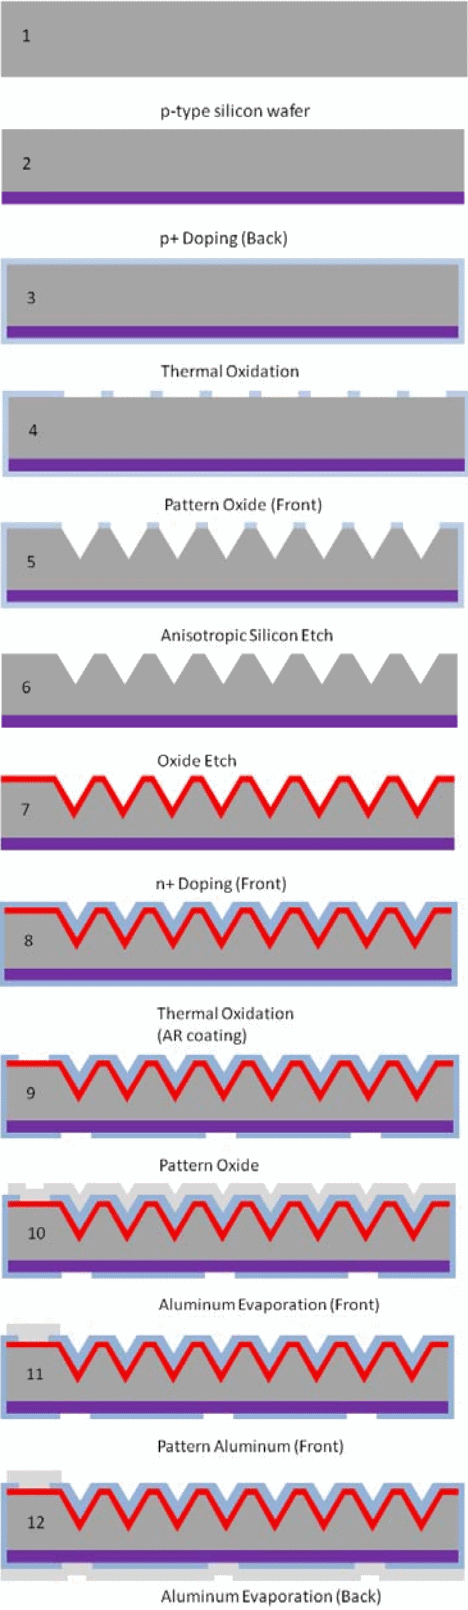
\includegraphics[height=.65\textheight]{./Images/Fabrication_Sequence.png}
			\caption{Fabrication Sequence for EELE408 Process \cite{408_Lab_Manual}}
			\label{fig:Fabrication_Sequence}
		\end{figure}
		
\FloatBarrier
\section{Measurements}
	\subsection{N+ Final Sheet Resistivity}
		The sheet resistivity of the N+ diffusion layer is measured during Lab 5, before the oxidation step. The measurements are shown in Table~\ref{tab:N+_Sheet_Resistivity}.  The average sheet resistivity is  64.2 $\Omega/\Box$.
		
		\begin{table}[h!]
			\centering
			\begin{tabular}{c || l | l | l }
				Direction	& Area 1	& Area 2	& Area 3	\\
				\hline
				FWD			& 67.4		& 62.4		& 61.3		\\
				\hline
				REV			& 66.7		& 66.1		& 66.6		\\
				\hline
			\end{tabular}
			\caption{N+ Sheet Resistivity in $\Omega/\Box$}
			\label{tab:N+_Sheet_Resistivity}
		\end{table}
	
	\subsection{P+ Final Sheet Resistivity}
		The sheet resistivity of the P+ diffusion layer is measured during Lab 2, before the oxidation step. The measurements are shown in Table~\ref{tab:P+_Sheet_Resistivity_1}.  The average sheet resistivity is 36.35 $\Omega/\Box$.
		
		\begin{table}[h!]
			\centering
			\begin{tabular}{c || l | l | l | l | l}
				Direction	& Area 1	& Area 2	& Area 3	& Area 4	& Area 5	\\
				\hline
				FWD			& 36.0		& 35.7		& 35.0		& 35.1		& 39.1	\\
				\hline
				REV			& 36.0		& 35.7		& 35.5		& 35.7		& 39.7	\\
				\hline
			\end{tabular}
			\caption{P+ Sheet Resistivity in $\Omega/\Box$}
			\label{tab:P+_Sheet_Resistivity_1}
		\end{table}
		
		After the N+ Diffusion, the sheet resistivity is measured again, as shown in Table~\ref{tab:P+_Sheet_Resistivity_2}.  The average sheet resistivity is 60.2 $\Omega/\Box$.
		
		\begin{table}[h!]
			\centering
			\begin{tabular}{c || l | l | l }
				Direction	& Area 1	& Area 2	& Area 3	\\
				\hline
				FWD			& 59.3		& 61.7		& 59.0		\\
				\hline
				REV			& 59.7		& 62.1		& 59.4		\\
				\hline
			\end{tabular}
			\caption{P+ Sheet Resistivity in $\Omega/\Box$}
			\label{tab:P+_Sheet_Resistivity_2}
		\end{table}
		
	\FloatBarrier
	\subsection{Front Al Sheet Resistivity}
		Using a four-point probe, the sheet resistivity of the front-side aluminum was measured to be 55 $m\Omega/\Box$.
	
	\subsection{Back Al Sheet Resistivity}
		Using a four-point probe, the sheet resistivity of the back-side aluminum was measured to be 60 $m\Omega/\Box$. 
	
	\subsection{Front Al Thickness}
		Figure~\ref{fig:Al_Thickness} shows the thickness of the aluminum on the front surface of the wafer after etching. The thickness of the patterned aluminum is measured using a profilometer. The elevation of the aluminum and silicon are both averaged to removed local maximums and minimums, leading to a measured thickness of 934 nm of aluminum.
		
		\begin{figure}[h!]
			\centering
			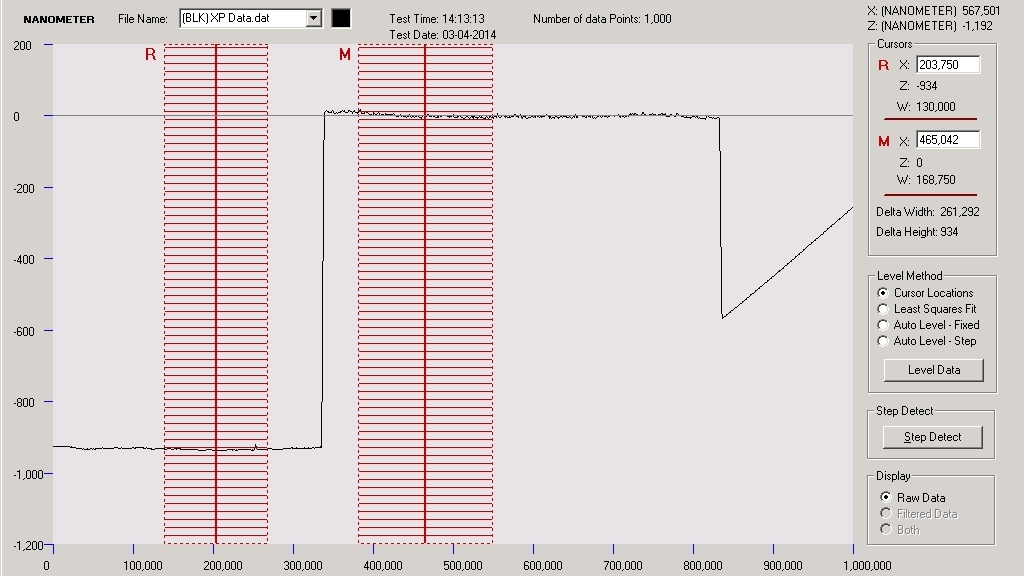
\includegraphics[width=.9\textwidth]{./Images/Harkness_Step.jpg}
			\caption{Aluminum Thickness}
			\label{fig:Al_Thickness}
		\end{figure}


\FloatBarrier
\section{Device Testing}

	Tables~\ref{tab:Before_Anneal} - \ref{tab:After_Cleave_2} contain the raw data collected from our measurements. Measurements were performed using a variable resistor and 2 multimeters, as shown in Figure~\ref{fig:Test_Setup}.
	
	\begin{figure}[h!]
		\centering
		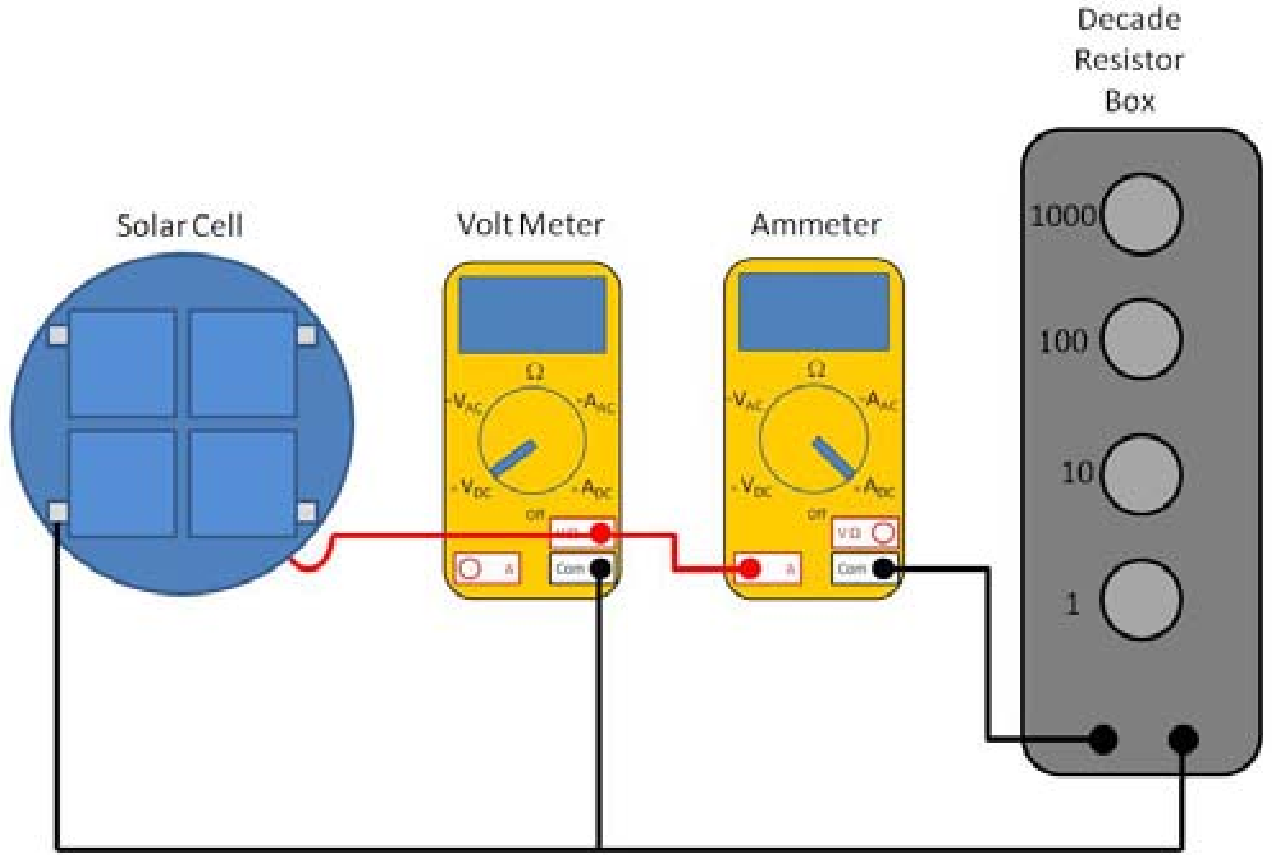
\includegraphics[width=.5\textwidth]{./Images/Test_Setup.png}
		\caption{Test Setup for IV measurements}
		\label{fig:Test_Setup}
	\end{figure}
	
	\begin{table}[h!]
		\centering
		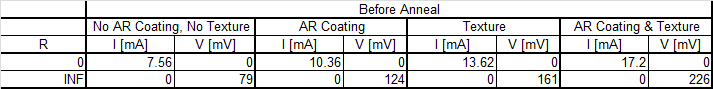
\includegraphics[width=.9\textwidth]{./Images/Tables/Before_Anneal.png}
		\caption{V$_{OC}$ and I$_{SC}$ before the anneal step}
		\label{tab:Before_Anneal}
	\end{table}
	
	\begin{table}[h!]
		\centering
		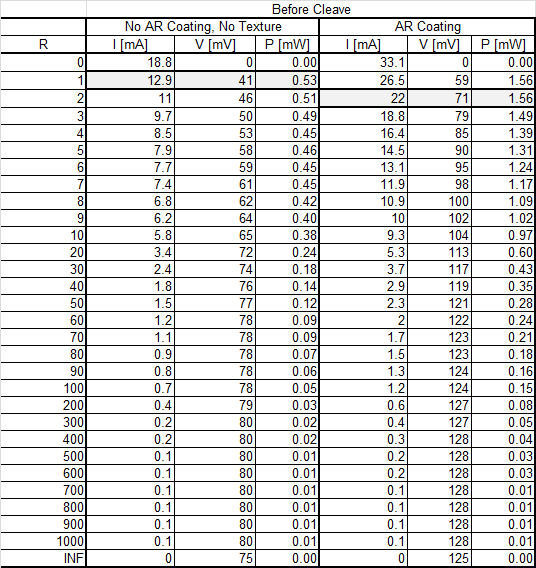
\includegraphics[width=.9\textwidth]{./Images/Tables/Before_Cleave_1.png}
		\caption{IV Measurements before cleaving the cells}
		\label{tab:Before_Cleave_1}
	\end{table}
	
	\begin{table}[h!]
		\centering
		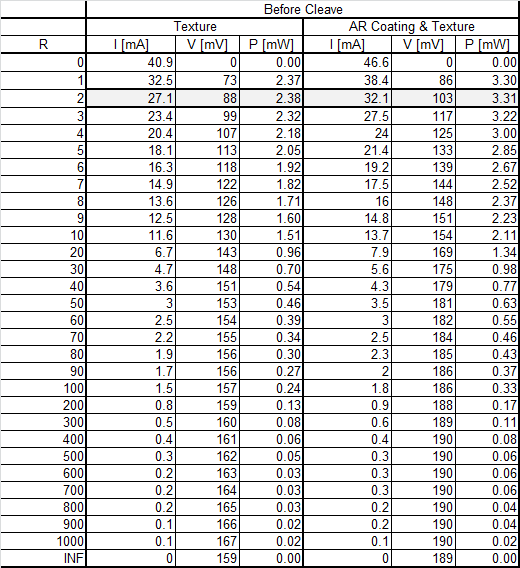
\includegraphics[width=.9\textwidth]{./Images/Tables/Before_Cleave_2.png}
		\caption{IV Measurements before cleaving the cells}
		\label{tab:Before_Cleave_2}
	\end{table}
	
	\begin{table}[h!]
		\centering
		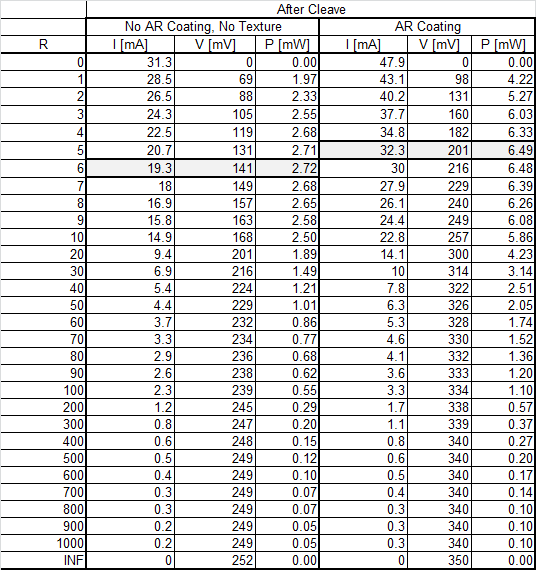
\includegraphics[width=.9\textwidth]{./Images/Tables/After_Cleave_1.png}
		\caption{IV Measurements after cleaving the cells}
		\label{tab:After_Cleave_1}
	\end{table}
	
	\begin{table}[h!]
		\centering
		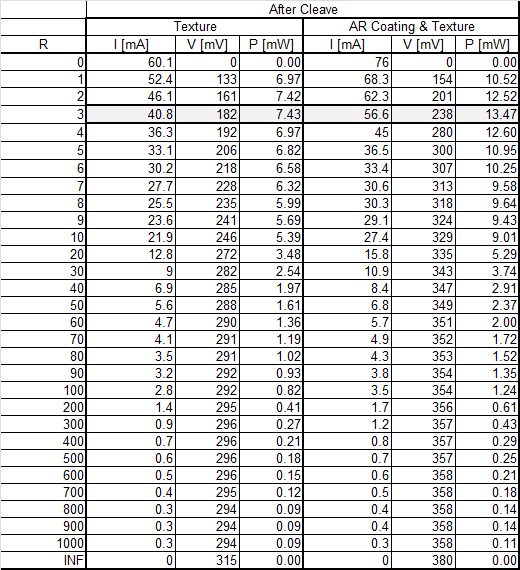
\includegraphics[width=.9\textwidth]{./Images/Tables/After_Cleave_2.png}
		\caption{IV Measurements after cleaving the cells}
		\label{tab:After_Cleave_2}
	\end{table}

\FloatBarrier
\section{Analysis}

	Figures~\ref{fig:Nothing} - \ref{fig:Both} show the IV and Power curves for each of our cells.  The three IV curves shown are: 
	\begin{itemize}
		\item taken immediately after depositing the back-side aluminum, before the anneal;
		\item after the anneal step;
		\item after the cells are separated and the side junction removed.
	\end{itemize}
	
	The series resistance of each cell is calculated as the slope of the IV curve near the open-circuit voltage $V_{OC}$, and the shunt resistance is calculated as the slope of the IV curve near the short-circuit current $I_{SC}$.
	
	The characteristic resistance each cell is calculated at the max power point.

	\begin{equation}
		R_{char} = \frac{V_{MP}}{I_{MP}}
	\end{equation}
	
	The Fill Factor of a solar cell is the ratio of the maximum power from the solar cell to the product of $V_{OC}$ and $I_{SC}$. Graphically, the FF is a measure of the "squareness" of the solar cell and is also the area of the largest rectangle which will fit in the IV curve.
	
	\begin{equation}
		FF = \frac{V_{MP} I_{MP}}{V_{OC} I_{SC}}
	\end{equation}
	
	The efficiency of a solar cell is the ratio of energy output from the solar cell to input energy from the sun.  Conditions under which efficiency is measured are carefully controlled to AM1.5 at a temperature of 25$^o$C.
	
	\begin{equation}
		\eta = \frac{V_{MP} I_{MP}}{P_{in}}
	\end{equation}

	AM1.5 translates to a power density of 1 kW/m$^2$. To determine the power being absorbed by the solar cell, the area of the solar cell must be calculated.  Each of our cells is 3.4 cm by 3.4 cm, resulting in an area of 1.1{\scriptsize E}-3 m$^2$. Using this, the power absorbed by the solar cell is 1.156 W.
	
	\pagebreak
	\FloatBarrier
	\subsection{No AR Coating, No Texturing}
	
		\begin{figure}[h!]
			\centering
			\begin{subfigure}[b]{.45\textwidth}
				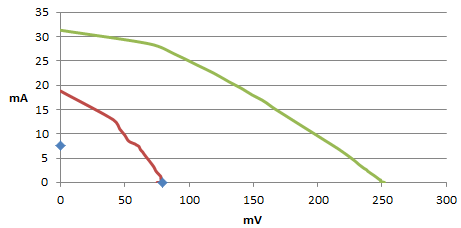
\includegraphics[width=\textwidth]{./Images/IV_Curves/Nothing_IV.png}
				\caption{IV Curves}
			\end{subfigure}
			~
			\begin{subfigure}[b]{.45\textwidth}
				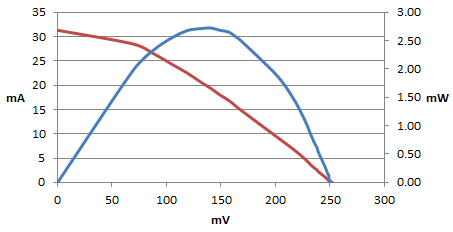
\includegraphics[width=\textwidth]{./Images/IV_Curves/Nothing_PV.png}
				\caption{Power Curve}
			\end{subfigure}
			
			\caption{No AR Coating, No Texture}
			\label{fig:Nothing}
		\end{figure}
		
		\begin{table}[h!]
			\centering
			\begin{tabular}{|c | r|}
				\hline
				R$_{series}$ [$\Omega$] & 5.164 \\
				\hline
				R$_{shunt}$ [$\Omega$] & 9.500 \\
				\hline
				R$_{char}$ [$\Omega$] & 7.306 \\
				\hline
				Fill Factor & 0.35 \\
				\hline
				Efficiency & 0.24\% \\
				\hline
			\end{tabular}
			\caption{No AR Coating, No Texture Parameters}
		\end{table}
		
	\FloatBarrier
	\subsection{AR Coating}
	
		\begin{figure}[h!]
			\centering
			\begin{subfigure}[b]{.45\textwidth}
				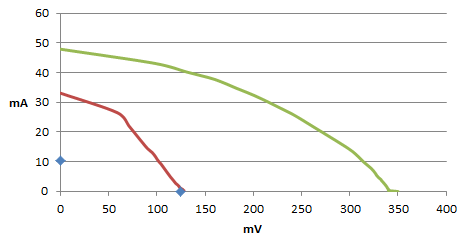
\includegraphics[width=\textwidth]{./Images/IV_Curves/AR_IV.png}
				\caption{IV Curves}
			\end{subfigure}
			~
			\begin{subfigure}[b]{.45\textwidth}
				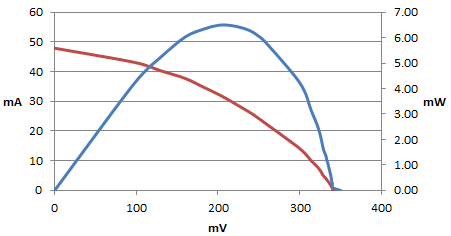
\includegraphics[width=\textwidth]{./Images/IV_Curves/AR_PV.png}
				\caption{Power Curve}
			\end{subfigure}
			
			\caption{AR Coating}
			\label{fig:AR_Coating}
		\end{figure}
		
		\begin{table}[h!]
			\centering
			\begin{tabular}{|c | r|}
				\hline
				R$_{series}$ [$\Omega$] & 2.822 \\
				\hline
				R$_{shunt}$ [$\Omega$] & 11.379 \\
				\hline
				R$_{char}$ [$\Omega$] & 6.223 \\
				\hline
				Fill Factor & 0.39 \\
				\hline
				Efficiency & 0.56\% \\
				\hline
			\end{tabular}
			\caption{AR Coating Parameters}
		\end{table}
		
	\FloatBarrier
	\subsection{Texturing}
	
		\begin{figure}[h!]
			\centering
			\begin{subfigure}[b]{.45\textwidth}
				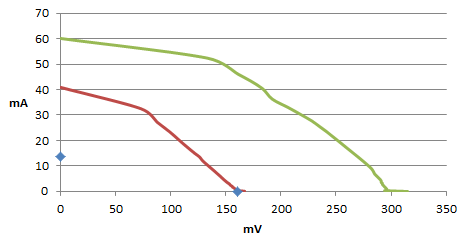
\includegraphics[width=\textwidth]{./Images/IV_Curves/Texture_IV.png}
				\caption{IV Curves}
			\end{subfigure}
			~
			\begin{subfigure}[b]{.45\textwidth}
				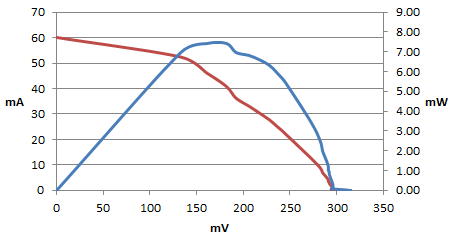
\includegraphics[width=\textwidth]{./Images/IV_Curves/Texture_PV.png}
				\caption{Power Curve}
			\end{subfigure}
			
			\caption{Texture}
			\label{fig:Texture}
		\end{figure}
		
		\begin{table}[h!]
			\centering
			\begin{tabular}{|c | r|}
				\hline
				R$_{series}$ [$\Omega$] & 1.798 \\
				\hline
				R$_{shunt}$ [$\Omega$] & 4.444 \\
				\hline
				R$_{char}$ [$\Omega$] & 4.461 \\
				\hline
				Fill Factor & 0.39 \\
				\hline
				Efficiency & 0.64\% \\
				\hline
			\end{tabular}
			\caption{Texture Parameters}
		\end{table}
	
	\FloatBarrier
	\subsection{AR Coating \& Texturing}
	
		\begin{figure}[h!]
			\centering
			\begin{subfigure}[b]{.45\textwidth}
				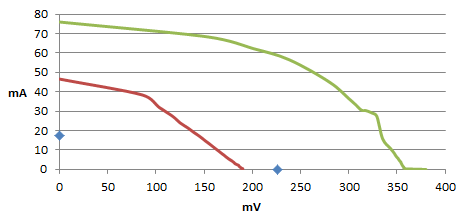
\includegraphics[width=\textwidth]{./Images/IV_Curves/Both_IV.png}
				\caption{IV Curves}
			\end{subfigure}
			~
			\begin{subfigure}[b]{.45\textwidth}
				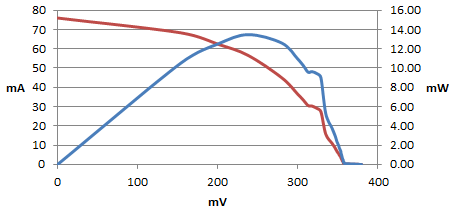
\includegraphics[width=\textwidth]{./Images/IV_Curves/Both_PV.png}
				\caption{Power Curve}
			\end{subfigure}
			
			\caption{AR Coating \& Texture}
			\label{fig:Both}
		\end{figure}
		
		\begin{table}[h!]
			\centering
			\begin{tabular}{|c | r|}
				\hline
				R$_{series}$ [$\Omega$] & 1.324 \\
				\hline
				R$_{shunt}$ [$\Omega$] & 7.833 \\
				\hline
				R$_{char}$ [$\Omega$] & 4.205 \\
				\hline
				Fill Factor & 0.47 \\
				\hline
				Efficiency & 1.17\% \\
				\hline
			\end{tabular}
			\caption{AR Coating \& Texture Parameters}
		\end{table}
		
	In all 4 cells, the anneal at least doubled I$_{SC}$, if not tripling it. V$_{OC}$ remained static, except in the case of the cell with both AR coating and texturing, where it decreased after the anneal.
	
	Of particular interest is the differences between the cells with AR coating and texturing.  They have nearly identical FF, but AR coating has a higher V$_{OC}$ and a respectively lower I$_{SC}$.
	
	It should be noted that these measurements were not performed under standard test conditions. The light source may not have been providing the expected 1kW/m$^2$. The copper backing plate was not being temperature controlled, with higher temperatures leading to reduced efficiencies.
	
	\subsection{Comparison of Class Data}
	Figures~\ref{fig:Alt_Nothing} - \ref{fig:Alt_Both} show the IV and Power curves for each of Tanner Whitlock's cells. Tanner's cells outperformed mine in most every case.  It is interesting to note that his cell with only AR coating actually outperforms the efficiency of his cell with both AR coating and texturing. The differences in our cell's operations are likely due to misalignments in photolithography, or better positioning in the oxidation and diffusion furnaces.
	
	
		\subsubsection{No AR Coating, No Texturing}
		
			\begin{figure}[h!]
				\centering
				\begin{subfigure}[b]{.45\textwidth}
					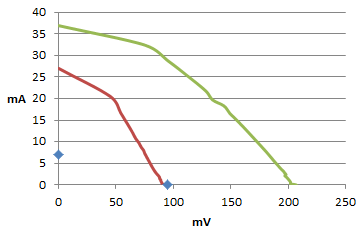
\includegraphics[width=\textwidth]{./Images/IV_Curves/Alt_Nothing_IV.png}
					\caption{IV Curves}
				\end{subfigure}
				~
				\begin{subfigure}[b]{.45\textwidth}
					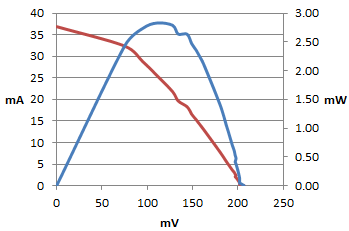
\includegraphics[width=\textwidth]{./Images/IV_Curves/Alt_Nothing_PV.png}
					\caption{Power Curve}
				\end{subfigure}
				
				\caption{No AR Coating, No Texture}
				\label{fig:Alt_Nothing}
			\end{figure}
			
			\begin{table}[h!]
				\centering
				\begin{tabular}{|c | r|}
					\hline
					R$_{series}$ [$\Omega$] & 3.132 \\
					\hline
					R$_{shunt}$ [$\Omega$] & 5.556 \\
					\hline
					R$_{char}$ [$\Omega$] & 4.353 \\
					\hline
					Fill Factor & 0.37 \\
					\hline
					Efficiency & 0.24\% \\
					\hline
				\end{tabular}
				\caption{No AR Coating, No Texture Parameters}
			\end{table}
			
		\FloatBarrier
		\subsubsection{AR Coating}
		
			\begin{figure}[h!]
				\centering
				\begin{subfigure}[b]{.45\textwidth}
					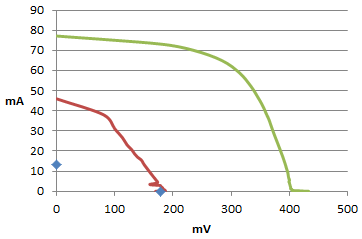
\includegraphics[width=\textwidth]{./Images/IV_Curves/Alt_AR_IV.png}
					\caption{IV Curves}
				\end{subfigure}
				~
				\begin{subfigure}[b]{.45\textwidth}
					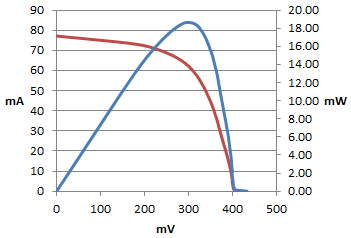
\includegraphics[width=\textwidth]{./Images/IV_Curves/Alt_AR_PV.png}
					\caption{Power Curve}
				\end{subfigure}
				
				\caption{AR Coating}
				\label{fig:Alt_AR_Coating}
			\end{figure}
			
			\begin{table}[h!]
				\centering
				\begin{tabular}{|c | r|}
					\hline
					R$_{series}$ [$\Omega$] & 0.945 \\
					\hline
					R$_{shunt}$ [$\Omega$] & 18.75 \\
					\hline
					R$_{char}$ [$\Omega$] & 5.331 \\
					\hline
					Fill Factor & 0.55 \\
					\hline
					Efficiency & 1.60\% \\
					\hline
				\end{tabular}
				\caption{AR Coating Parameters}
			\end{table}
		
		\pagebreak
		\FloatBarrier
		\subsubsection{Texturing}
		
			\begin{figure}[h!]
				\centering
				\begin{subfigure}[b]{.45\textwidth}
					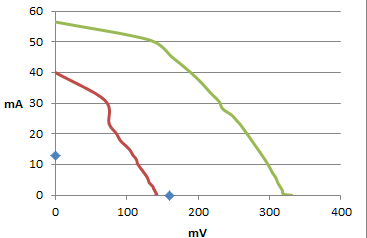
\includegraphics[width=\textwidth]{./Images/IV_Curves/Alt_Texture_IV.png}
					\caption{IV Curves}
				\end{subfigure}
				~
				\begin{subfigure}[b]{.45\textwidth}
					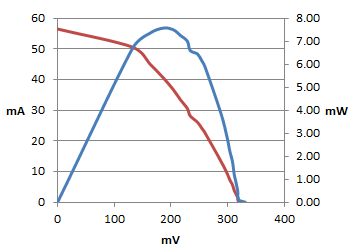
\includegraphics[width=\textwidth]{./Images/IV_Curves/Alt_Texture_PV.png}
					\caption{Power Curve}
				\end{subfigure}
				
				\caption{Texture}
				\label{fig:Alt_Texture}
			\end{figure}
			
			\begin{table}[h!]
				\centering
				\begin{tabular}{|c | r|}
					\hline
					R$_{series}$ [$\Omega$] & 2.603 \\
					\hline
					R$_{shunt}$ [$\Omega$] & 5.636 \\
					\hline
					R$_{char}$ [$\Omega$] & 4.617 \\
					\hline
					Fill Factor & 0.40 \\
					\hline
					Efficiency & 0.66\% \\
					\hline
				\end{tabular}
				\caption{Texture Parameters}
			\end{table}
		
		\FloatBarrier
		\subsubsection{AR Coating \& Texturing}
		
			\begin{figure}[h!]
				\centering
				\begin{subfigure}[b]{.45\textwidth}
					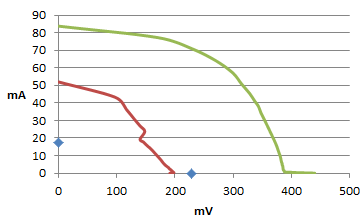
\includegraphics[width=\textwidth]{./Images/IV_Curves/Alt_Both_IV.png}
					\caption{IV Curves}
				\end{subfigure}
				~
				\begin{subfigure}[b]{.45\textwidth}
					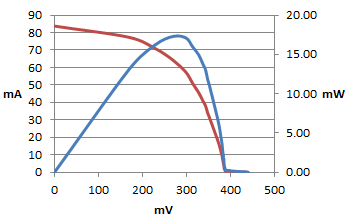
\includegraphics[width=\textwidth]{./Images/IV_Curves/Alt_Both_PV.png}
					\caption{Power Curve}
				\end{subfigure}
				
				\caption{AR Coating \& Texture}
				\label{fig:Alt_Both}
			\end{figure}
			
			\begin{table}[h!]
				\centering
				\begin{tabular}{|c | r|}
					\hline
					R$_{series}$ [$\Omega$] & 1.516 \\
					\hline
					R$_{shunt}$ [$\Omega$] & 9.219 \\
					\hline
					R$_{char}$ [$\Omega$] & 4.212 \\
					\hline
					Fill Factor & 0.47 \\
					\hline
					Efficiency & 1.50\% \\
					\hline
				\end{tabular}
				\caption{AR Coating \& Texture Parameters}
			\end{table}
	

\FloatBarrier
\section{Summary}
	\subsection{Results}
		As expected, the cell with an AR coating and texturing outperformed all the other cells in almost every way.  It has the highest V$_{OC}$, I$_{SC}$, P$_{MP}$, Fill Factor, and Efficiency.
		
		All the cells though perform terribly compared to commercial and researched produced PV cells.  Compared to a textbook IV curve, our cells begin to drop current far faster.  This is due to a lower shunt resistance than normal. This could imply that not enough material was filed off the edge of each cell, but may just be due to a poor PN junction.
	
	\subsection{Recommendations}
		I personally prefer a physical textbook to a website or slides, and would be willing to purchase a textbook off of Amazon as opposed to the MSU bookstore.
		
\pagebreak
\printbibliography

\end{document}